\documentclass[conference,compsoc]{IEEEtran}
\usepackage{cite}
\usepackage{listings}
\usepackage{blindtext}
\usepackage{enumitem}
% for coding highlight
\usepackage{graphicx}
\usepackage[colorlinks=true,urlcolor=blue]{hyperref}
\usepackage{amsmath, amsthm, amssymb}
\usepackage{subfloat}
\usepackage{ulem}
\usepackage{indentfirst}
\usepackage{booktabs}
\usepackage{wrapfig,lipsum,booktabs}
\usepackage{array}
\usepackage{ulem}
\usepackage{indentfirst}
\usepackage{listings}
\usepackage{color}
\definecolor{codegreen}{rgb}{0,0.6,0}
\definecolor{codegray}{rgb}{0.5,0.5,0.5}
\definecolor{codepurple}{rgb}{0.58,0,0.82}
\definecolor{backcolour}{rgb}{0.95,0.95,0.92}


\lstdefinestyle{mystyle}{
    backgroundcolor=\color{backcolour},   
    commentstyle=\color{codegreen},
    keywordstyle=\color{magenta},
    numberstyle=\tiny\color{codegray},
    stringstyle=\color{codepurple},
    basicstyle=\footnotesize,
    breakatwhitespace=false,         
    breaklines=true,                 
    captionpos=b,                    
    keepspaces=true,                 
    numbers=left,                    
    numbersep=5pt,                  
    showspaces=false,                
    showstringspaces=false,
    showtabs=false,                  
    tabsize=2
}
\lstset{style=mystyle}

\newcommand{\subparagraph}{}
\newcolumntype{C}[1]{>{\centering\let\newline\\\arraybackslash\hspace{0pt}}m{#1}}

\begin{document}
\title{
	Deep Learning Course Proposal \\
	Passenger Screening Algorithm Challenge \\
}


% author names and affiliations
% use a multiple column layout for up to three different
% affiliations
\author{
	\IEEEauthorblockN{Yuyang Rong}
	\IEEEauthorblockA{
		School of Information Science and Technology \\
		ShanghaiTech University \\
		Student ID: 69850764 \\
	}
\and
	\IEEEauthorblockN{Peng Ding}
	\IEEEauthorblockA{
		School of Information Science and Technology \\
		ShanghaiTech University \\
		Student ID: 79406120 \\
	}
}

\maketitle

\section{Problem Description}
	\par The safety issue has always been a major concern since the day that aviation was civilized. Detecting whether passengers are carrying any prohibited items is one of the key steps before passenger board the plane. Conventionally, passengers are required to be screened and physically examined by TSA staffs. Such procedure takes time and effort to operate, without guaranteeing the accuracy of checking. Whereas complaints call upon the invasion of personal privacy. With all these being considered, people rarely consider the traditional security check as a satisfactory experience. We propose a computer vision approach, utilizing deep learning method by examining critical positions of human gestures, to facilitate with the detection of prohibited items.
	\par To tackle this problem, first we have to partition human bodies into 17 parts, see \ref{bodyzones}
	\begin{figure} \label{bodyzones}
		\centering
		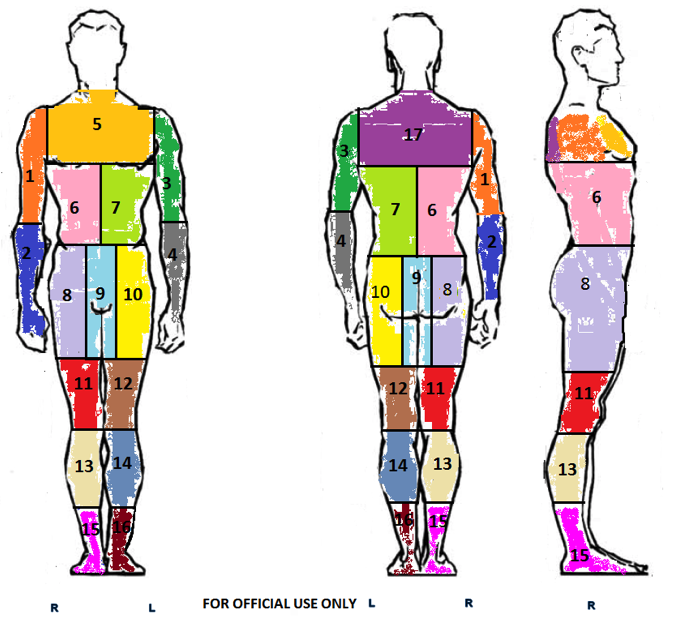
\includegraphics[width=\linewidth]{./Pic/body_zones}
		\caption{17 zones of human body.}
	\end{figure}
	\par We are given scans of one person, each scan have 22.5 degrees difference, thus in total we have 16 images per person. Each image has resolution 512*660. 
	
\section{Data Preprocessing}
	\subsection{Image Crop}
		\par We have considered the possibility of taking 512*660*16 images as input and a vector of size 17*1 describing the possibility of presence of dangerous objects. However, considering there isn't much positive outcomes, we decided to crop the images and for each zone, only see certain sector of the image.
		\par The image is cropped into 16 sectors, each sector has size 250*250 pixels. The table listed the upper left conner of each sector:
		\begin{table}[h]
			\centering
			\caption{My caption}
			\label{my-label}
			\begin{tabular}{ccc}
				\hline
				Region \# & x   & y   \\ \hline
				1         & 50  & 50  \\ \hline
				2         & 0   & 0   \\ \hline
				3         & 50  & 250 \\ \hline
				4         & 250 & 0   \\ \hline
				5         & 150 & 150 \\ \hline
				6         & 200 & 100 \\ \hline
				7         & 200 & 150 \\ \hline
				8         & 250 & 50  \\ \hline
				9         & 250 & 150 \\ \hline
				10        & 300 & 200 \\ \hline
				11        & 400 & 100 \\ \hline
				12        & 350 & 200 \\ \hline
				13        & 410 & 0   \\ \hline
				14        & 410 & 200 \\ \hline
				15        & 410 & 0   \\ \hline
				16        & 410 & 200 \\ \hline
			\end{tabular}
			\caption{Region distribution.}
		\end{table}
	\subsection{Zone assignment}
		\par Now that we have already cropped each image, we will assign each region to it's zones. This makes recognition on each zone easier. Now that no zone can be shown in all 16 images, we will represent it by a None in python.
		\par We have done the pre-calculation to assign sectors based on the index of the image. For example, threat zone 1(Right Bicep) can be see in sector 1 in image 0, 1, 2, 13, 14, 15; in sector 3 in image 6 to 10. Thus in python we write:
		\begin{lstlisting}[language = python]
zone_slice_list = [ [ # threat zone 1
   sector01_pts, sector01_pts, sector01_pts, None, None, None, sector03_pts, sector03_pts, sector03_pts, sector03_pts, sector03_pts, None, None, sector01_pts, sector01_pts, sector01_pts ],
   # To be continued.
]
		\end{lstlisting}
	\subsection{Up Sample}
		\par For the data set given for now, there are 1871 positive outcomes over 19500 samples, distributed all over 17 zones. This made our work harder because deep learning algorithms will be looking for more positive outcomes to learn. 
		\par We are up sampling the positive outcomes by duplicate positive outcomes and mirror positive images. Thus we will be having more than 5000 positive images. It's unclear whether this is enough, 
\section{Approach}
	\par Now that we have cropped each image and assigned them to 17 zones. We can tackle each zones once at a time. We will build a network for all zones and then train/test them separately.

\section{Deep Neural Tricks}
	\par We have been investigating tricks we can use for deep neural so that we can train faster.
\bibliographystyle{IEEEtran}
%% De-comment this line if you have any reference.
%% And don't forget to change .bib file.
% \bibliography{milestone}
\end{document}
